\documentclass[10pt,a4paper]{article}


% Packages laden
\usepackage[a4paper,top=3cm,bottom=2cm,left=2cm,right=2cm]{geometry}		% paginagrootte
%\usepackage{a4wide}
\usepackage{parskip}									% andere regels voor nieuwe paragraaf: witregel + niet inspringen

\usepackage[english]{babel}						%	spelling en woordafbreking (Engles)
\usepackage[latin1]{inputenc}					% invoer van speciale tekens (bvb. Umlaut)
\usepackage[T1]{fontenc}							% weergave van speciale tekens (bvb. Umlaut)
\usepackage{lmodern}									% betere weergave van speciale tekens (bvb. Umlaut)
%\usepackage{dsfont}	
\usepackage{amsfonts,amsthm, tabularx}					% wiskundige symbolen and table of equations
%\usepackage[fleqn]{amsmath}
\usepackage{graphicx}
\usepackage{epstopdf}

% Package for hyperlink, without ugly box around and nice blue color for text
\usepackage{hyperref}
\usepackage{xcolor}
\hypersetup{
    colorlinks,
    linkcolor={red!50!black},
    citecolor={blue!50!black},
    urlcolor={blue!80!black}
}

\usepackage{graphicx}
\usepackage{caption}
\usepackage{subcaption}

\usepackage{float}										% plaatsen van figuren en tabellen
\usepackage[format=plain,
						indent=1cm]{caption}			% personaliseren van onderschriften
\usepackage{eurosym}									% sign of euro

% Instellingen voor document
\renewcommand{\arraystretch}{1.1}			% tabelrijen iets hoger maken

\usepackage{amsmath,amsfonts,amsthm,mathrsfs,MnSymbol}	% wiskundige symbolen
\renewcommand*\thesection{\arabic{section}}
\DeclareMathOperator*{\argmin}{\arg\!\min}
\usepackage{pifont}							

\setcounter{secnumdepth}{3}		% Enable subsubsection numbering
\setcounter{tocdepth}{3}		% Include subsubsection in table of content

\usepackage{color}				% Load the color package: \color{declared-color}{text}. If also background:
								% \colorbox{declared-color1}{\color{declared-color2}text}
%Aangepaste header
\usepackage{fancyhdr}
\pagestyle{fancyplain}
\renewcommand{\headrulewidth}{1.0pt}
\lhead{\fancyplain{}{Crash course Modelica}}
\rhead{\fancyplain{}{\today}}

\usepackage{listings}
\usepackage{siunitx}
%% listings-modelica.cfg
%% Copyright 2014 Martin Sjoelund, Dietmar Winkler
%
% This work may be distributed and/or modified under the
% conditions of the LaTeX Project Public License, either version 1.3
% of this license or (at your option) any later version.
% The latest version of this license is in
%   http://www.latex-project.org/lppl.txt
% and version 1.3 or later is part of all distributions of LaTeX
% version 2005/12/01 or later.
%
% This work has the LPPL maintenance status `maintained'.
%
% The Current Maintainer of this work is Dietmar Winkler
%
% Code repository https://github.com/modelica-tools/listings-modelica
%
% This work consists of the file listings-modelica.cfg

\lstdefinelanguage{modelica}
{
  morekeywords=[1]{
    algorithm,and,annotation,as,assert,block,break,case,class,connect,connector,
    constant,constrainedby,der,discrete,each,else,elseif,elsewhen,encapsulated,
    end,enumeration,equality,equation,expandable,extends,external,failure,final,
    flow,for,function,guard,if,import,in,initial,inner,input,List,local,loop,
    match,matchcontinue,model,not,operator,Option,or,outer,output,package,parameter,
    partial,protected,public,record,redeclare,replaceable,return,stream,
    subtypeof,then,Tuple,type,uniontype,when,while},
  morekeywords=[2]{true, false},
  % Do not make true,false keywords because fn(true,x, false ) shows up as fn(true,x, *false*)
  morekeywords=[3]{optimization,constraint}, % Optimica keywords
  morekeywords=[4]{objective,startTime,finalTime,initialGuess},
  sensitive=true,
  comment=[l]//,
  morecomment=[s]{/*}{*/},
  alsodigit={.,-},
  morestring=[b]',
  morestring=[b]",
}[keywords,comments,strings]

\definecolor{keywordcolor1}{rgb}{0,0,.4}
\definecolor{keywordcolor2}{rgb}{.90,0,0}
\definecolor{keywordcolor3}{rgb}{.4,0,.8}
\definecolor{keywordcolor4}{rgb}{0.5,0,0.5}
\definecolor{stringcolor}{rgb}{0.133,0.545,0.133}
% \definecolor{listingbgcolor}{rgb}{0.95,0.95,0.95}

\lstset{
  breaklines=true,
  language=modelica,
  basicstyle=\ttfamily,
  keywordstyle=[1]\color{keywordcolor1}\bfseries,
  keywordstyle=[2]\color{keywordcolor2},
  keywordstyle=[3]\color{keywordcolor3}\bfseries,
  keywordstyle=[4]\color{keywordcolor4},
  stringstyle=\color{stringcolor},
%  backgroundcolor=\color{listingbgcolor},
  framexleftmargin=5pt,
  xleftmargin=5pt,
  xrightmargin=5pt,
  showstringspaces=false
}

\newcommand{\code}[1]{\lstinline|#1|}
\newcommand{\modelica}[1]{\lstinline[language=modelica]|#1|}


\author{Bram van der Heijde}
						
\begin{document}

\section*{Prepare for the Modelica Crash Course!}

This guide will help you to install Dymola and already get the hang of Modelica, such that you can profit maximally from the Crash Course. 

\subsection*{Installation}

First of all, install Dymola (commercial software).  Fill out this 
\href{http://www.claytex.com/products/dymola/dymola-demo/}{form} to download 
the demo. After installation you HAVE to install a c-compiler, otherwise you 
cannot run any model.  You can download and install for example the Visual 
Studio \texttt{C++} 2017 Build Tools from this  
\href{https://visualstudio.microsoft.com/thank-you-downloading-visual-studio/?sku=BuildTools&rel=15}{link}.
Do not forget to select your C-compiler in \texttt{Dymola>Simulation Set 
Up>Compiler}. 
In order to access this menu item, open Dymola and change to the Simulation tab 
(lower right corner).
Test your installation by running a demo (e.g. open File/Demos/Robot, then 
click Commands/Simulate and wait till you see a graph). 
More detailed 
instructions can be found 
\href{https://www.3ds.com/fileadmin/PRODUCTS/CATIA/DYMOLA/PDF/Installation.pdf}{here}.

\subsection*{Prerequisites}
Read the following chapters of the open-access book  
\href{http://book.xogeny.com/}{Modelica by Example} of Michael M. Tiller 
carefully.

\begin{enumerate}
\item \href{http://book.xogeny.com/behavior/equations/}{Basic equations}: general introduction to the Modelica language, illustration of the model structure, basic concepts such as derivative, initialization, parameter, variable and type.
\item \href{http://book.xogeny.com/behavior/functions/polynomial/}{Polynomial 
Evaluation}: Example of 
\href{http://book.xogeny.com/behavior/functions/func_def/}{function 
definition}, protected variable and time.
\item \href{http://book.xogeny.com/behavior/arrays/oned/}{One-Dimensional Heat Transfer}: introduction to arrays and loop in Modelica.
\item	\href{http://book.xogeny.com/components/connectors/}{Connectors}: Component-Oriented Modeling, classes of variables.



\end{enumerate}

Carefully read chapter 1 ``What is Dymola?'' (p.~13 to 22) of the Dymola manual 
Volume 1 (can be found in your installation folder: C:\textbackslash Program 
Files (x86)\textbackslash Dymola \textit{xx}\textbackslash Documentation 
\textbackslash Dymola User Manual Volume 1, where \textit{xx} stands for the 
version you installed) to get familiar with the Dymola environment (model 
editor, parameters change, simulation, ...).\\

For further background, following sections from ``Modelica by Example'' of 
Michael Tiller are interesting, however it is not compulsory to read before the 
course: 
\begin{enumerate}
\item \href{http://book.xogeny.com/behavior/discrete/}{Discrete Behavior} >State Event Handling, Hysteresis and Review
\item	\href{http://book.xogeny.com/behavior/arrays/}{Vectors and Arrays} >Array Declarations and Array Construction
\item	\href{http://book.xogeny.com/components/components/#review}{Components}>Review, Examples>Heat Transfer Components, Electrical Components
\item \href{http://book.xogeny.com/components/architectures/replaceable/}{Architecture>Configuration Management}
		
\end{enumerate}

\subsection*{Homework exercise}
The purpose of this exercise is to model an electrical circuit using only your own code implementation. You will learn how to create connectors, partial models, models and how to re-use your code.

\begin{figure}[h]
	\centering
	\begin{minipage}{.4\textwidth}
		\centering
		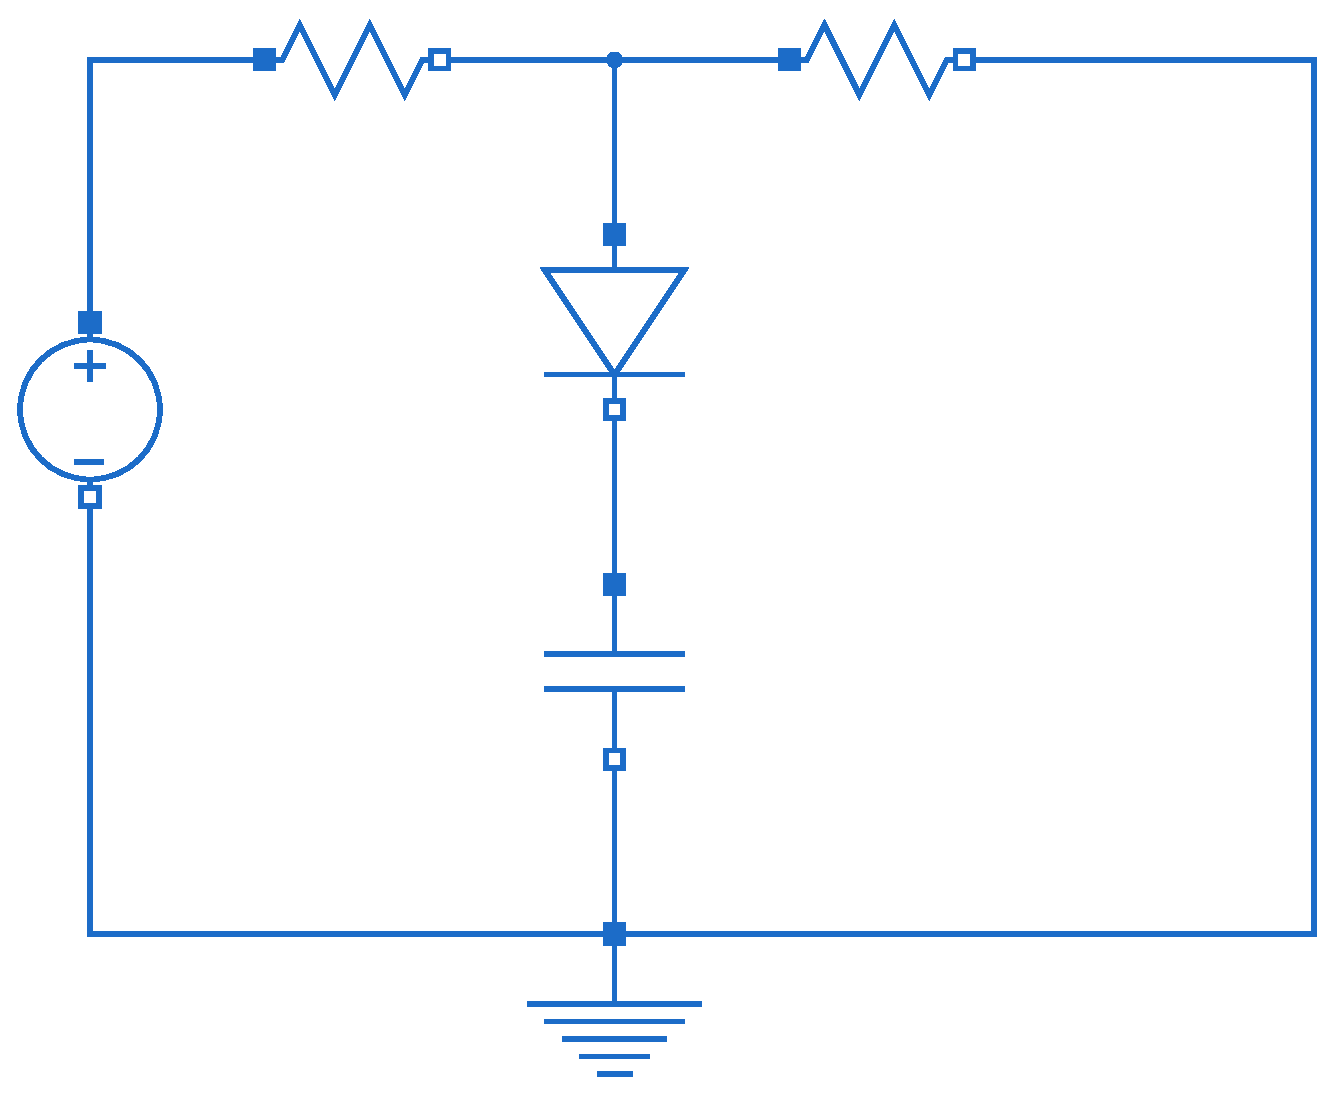
\includegraphics[width=1\linewidth]{images/circuit.eps}
		\captionof{figure}{Electrical circuit.}
		\label{fig:cir}
	\end{minipage}%
	\begin{minipage}{.6\textwidth}
		\centering
		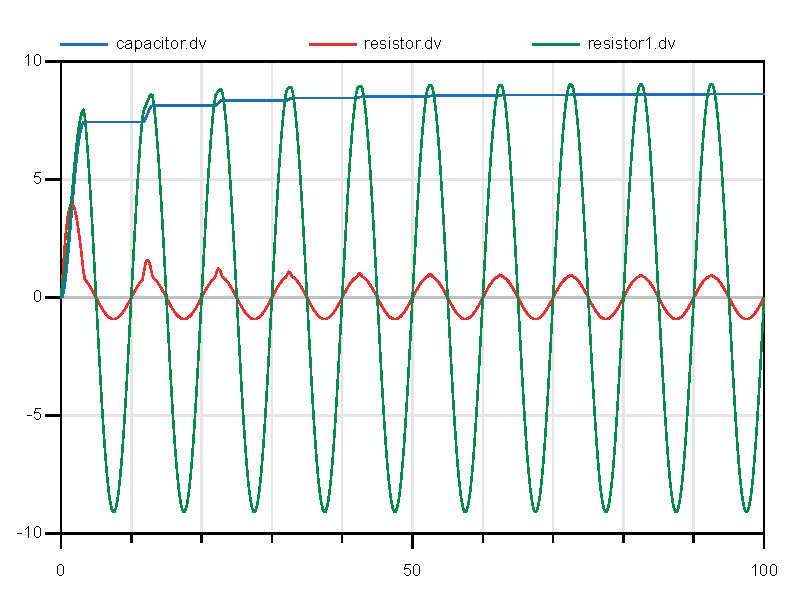
\includegraphics[width=.8\linewidth]{images/result.eps}
		\captionof{figure}{Result of simulation}
		\label{fig:res}
	\end{minipage}
\end{figure}


Consider the electrical circuit shown in Fig.~\ref{fig:cir}. The circuit has a 
sinusoidal source, a resistor, a diode, a capacitor and the ground. You are 
going to build your first Modelica library from scratch to compose this model.

Some tips:
\begin{itemize}
	\item Make sure you end statements in Modelica code with a semicolon 
	(\textbf{;}). With some exceptions (e.g., \texttt{(partial) model}, 
	\texttt{equation} and \texttt{algorithm} lines), this is always necessary.
	\item You can \texttt{check} your model using the check box in the toolbar. 
	This will usually point you to possible mistakes you made, so make sure to 
	read error and warning messages carefully. Although Modelica has a bad 
	reputation for debugging, its syntax checker is not bad.
	\item Dymola has a nifty autocompletion function, which helps you reduce 
	how much of the code you have to type yourself. Just start typing something 
	and press \texttt{Ctrl + space} to open a context menu with some 
	suggestions.
\end{itemize}


\begin{enumerate}
	\item After opening Dymola, create a new \textit{package} called 
	\textit{MyLib} (through \texttt{File>New>Package\ldots}). Don't forget to 
	provide an appropriate description so you know what your library is for 
	when you don't touch it for a longer time. Also, it is useful to deselect 
	``Save contents of package in one file'' if you are going to use version 
	control (GIT).
	
	All component models you will define in the following step need to be 
	placed in this folder.
	
	\item Each component uses electrical connectors. Create a \texttt{partial 
	connector} (right-click \textit{MyLib}, then \texttt{New > 
	Connector\ldots}). Make sure to select the option ``Partial'' in the dialog 
	that pops up.
	Call the \texttt{partial connector} \textit{Pin}. This connector will need 
	two variables $i$ (current) and $v$ 
	(voltage). You can add variables while you are in the \textit{Modelica 
	text} context of the \textit{Modeling} tab. If you want to know how to 
	create variables in the \texttt{Modelica text} context, you can review 
	\href{http://book.xogeny.com/behavior/equations/variables/#variables}{this 
	page}. 

	Which one is a \textit{flow} and which is a \textit{potential} variable, 
	and how should this be reflected in your code? Check 
	\href{http://book.xogeny.com/components/connectors/simple_domains/#simple-domains}{this
	 link} for a hint.
	
	\item Create the \texttt{connector}s \textit{Pin\_a} and \textit{Pin\_b} 
	for the positive and negative pins.  Use \texttt{extends} to inherit the 
	variables $i$ and $v$ from the \texttt{partial connector} you have just 
	defined. 
	An easy way to create extending models is by right-clicking on the model 
	you want to extend from, and click \texttt{New > Extend from\ldots}.
	
	Make two different graphical illustrations for the pins. To do so, select 
	the \texttt{Icon} context from the toolbar. For example, you can draw a 
	square in the available canvas and choose a different color for each of the 
	pins. A good convention is to use the same shape for pins of the same flow 
	type. 
	
	\item Create a \texttt{partial model} \textit{OnePin} which contains the 
	variables $i$ (current) and $v$ (voltage) and one connector 
	\textit{Pin\_a}. To add the connector, drag \textit{Pin\_a} from your 
	libary folder to the modelling window while you are in the \textit{Diagram} 
	context of the \textit{Modeling} tab. The pin should be located on the top 
	border of the white canvas. This model will be the basis for all models 
	which have only one pin (i.e. the ground node).
	
	\item Create variables $i$ and $v$ in \textit{OnePin} and write 
	\texttt{equation}s to link these variables to those you have defined in the 
	\textit{Pin} you use in the component. In order to access variables, you 
	can use dot notation as follows: \texttt{componentName.variable}.
	
	Your code should look something like this:
	\begin{lstlisting}
	partial model OnePin "Model with a single pin"
	  flow Modelica.SIunits.Current i "Current flowing through this component";
	  Modelica.SIunits.Voltage v "Voltage of this component";
	
	  Pin_a pin annotation...;
	equation
	  pin.i = i;
	  pin.v = v;
	  annotation...;
	end OnePin;
	\end{lstlisting}
	
	Notice that the model \texttt{OnePin} contains an instance of 
	\texttt{Pin\_a} named \texttt{pin}. In the \texttt{equation} section, you 
	can see that the current through this \texttt{pin} is accessed with the 
	dot-notation and made equal to the current of the \texttt{OnePin}. The same 
	is done for the voltages. \\
	However, it is not possible to access a variable on something that is not 
	an instance of a Modelica model. For instance, \texttt{OnePin.v} would make 
	no sense.
	
	\item Now create a \texttt{partial model} \textit{TwoPin} with the same 
	variables and two \textit{Pin} connectors, one positive pin on the left and 
	one negative on the right. Add two variables: voltage difference between 
	the two pins $dv$ and current $i$. 
	While still in \texttt{partial model} \textit{TwoPin}, add equations that link the variables in this model with the variables of the pins. When connecting currents, use the convention that when the current flows into the component from the pin, it is positive and vice versa.
	
	\item Create the source, the resistor, the diode and the capacity by extending \textit{OnePin} or \textit{TwoPin}. Make use of the following equations:
	\begin{enumerate}
		\item Resistor: $R i = v$\footnote{$v$ in this equation is equivalent to variable $dv$ in the Modelica model.}
		\item Capacity: $C \frac{d v}{dt} = i$
		\item source: $v = V sin( 2 \pi f t + \omega) + \beta$
		\item Diode: if $ \frac{v}{V_t} \geq \alpha$: $i = I_{ds} \left( \exp\left(\alpha \left( 1 + \frac{v}{V_t} - \alpha \right)\right) - 1\right) + \frac{v}{R}$, else $i = I_{ds} (e^\alpha - 1) + \frac{v}{R}$
		\item ground: $ v = 0$
	\end{enumerate}
	Define $R$, $C$,\ldots as \texttt{parameter}, such that you can change their value using the parameter dialog in the \textit{Diagram} context.\\
	Make use of following values for the diode: $I_{ds}$ = 1.e-6, $V_t=0.04$, 
	$\alpha=1$, $R=1.e8$.
	To review how to define the time derivative of a variable, revise 
	\href{http://book.xogeny.com/behavior/equations/first_order/}{this link}.
	\item Create a model called \textit{Circuit} in which you include all these 
	components as shown in Fig.~\ref{fig:cir}.
	
	You are very welcome to experiment with model parameters, but to verify 
	your solution against Fig.~\ref{fig:res}, use following parameters:
	\begin{itemize}
		\item Voltage source: frequency \SI{0.1}{\hertz}, voltage \SI{10}{\volt}
		\item Left resistance: Resistance \SI{1}{\ohm}
		\item Right resistance: Resistance \SI{10}{\ohm}
		\item Diode: as indicated above
		\item Capacitor: Capacity \SI{1}{\farad}, start voltage \SI{0}{\volt}
	\end{itemize}
	\item Simulate the circuit for 100 seconds.
\end{enumerate}

\subsection*{Optional exercise}
This assignment aims at testing your comprehension of the basic Modelica concepts learned during the above mentioned reading by setting a model of a building and simulating its thermal behaviour. \textbf{This assignment will not be treated during the Crash Course. However, you may find it a useful exercise to get more acquainted with Modelica and Dymola.}

Let us consider a simplified building as represented in Fig. \ref{fig:bui}. The building consists of  walls, a window and a single room called \textit{zone} which thermally interacts with the environment(ambient air \textit{TAmb}, the ground, and the sun. The building foundation is approximated by a thick concrete layer called \textit{slab} separating the zone from the ground. On the right-hand side of the figure, a thermal model of the building is proposed using the resistance-capacitance approach. The heat transfer is approximated by a 1D conduction resistance and the heat storage by a heat capacity. \textit{CZone} represents the thermal capacity of the zone (consisting of the internal walls, the furnitures, and a part of the external wall). The \textit{CSlab}'s represent the thermal capacities of the slab. Finally, the ground is discretized in \textit{n = 5} layers, each of them having an identical heat capacity \textit{CGro[i]}. Through the window, the sun heats up the room with a thermal power $QSol$. 

The value of the parameters is given in Table \ref{tab:par}. Using the electrical analogy, the governing equations of the system are the following:

\begin{figure}[hbtp] 
	\centering
	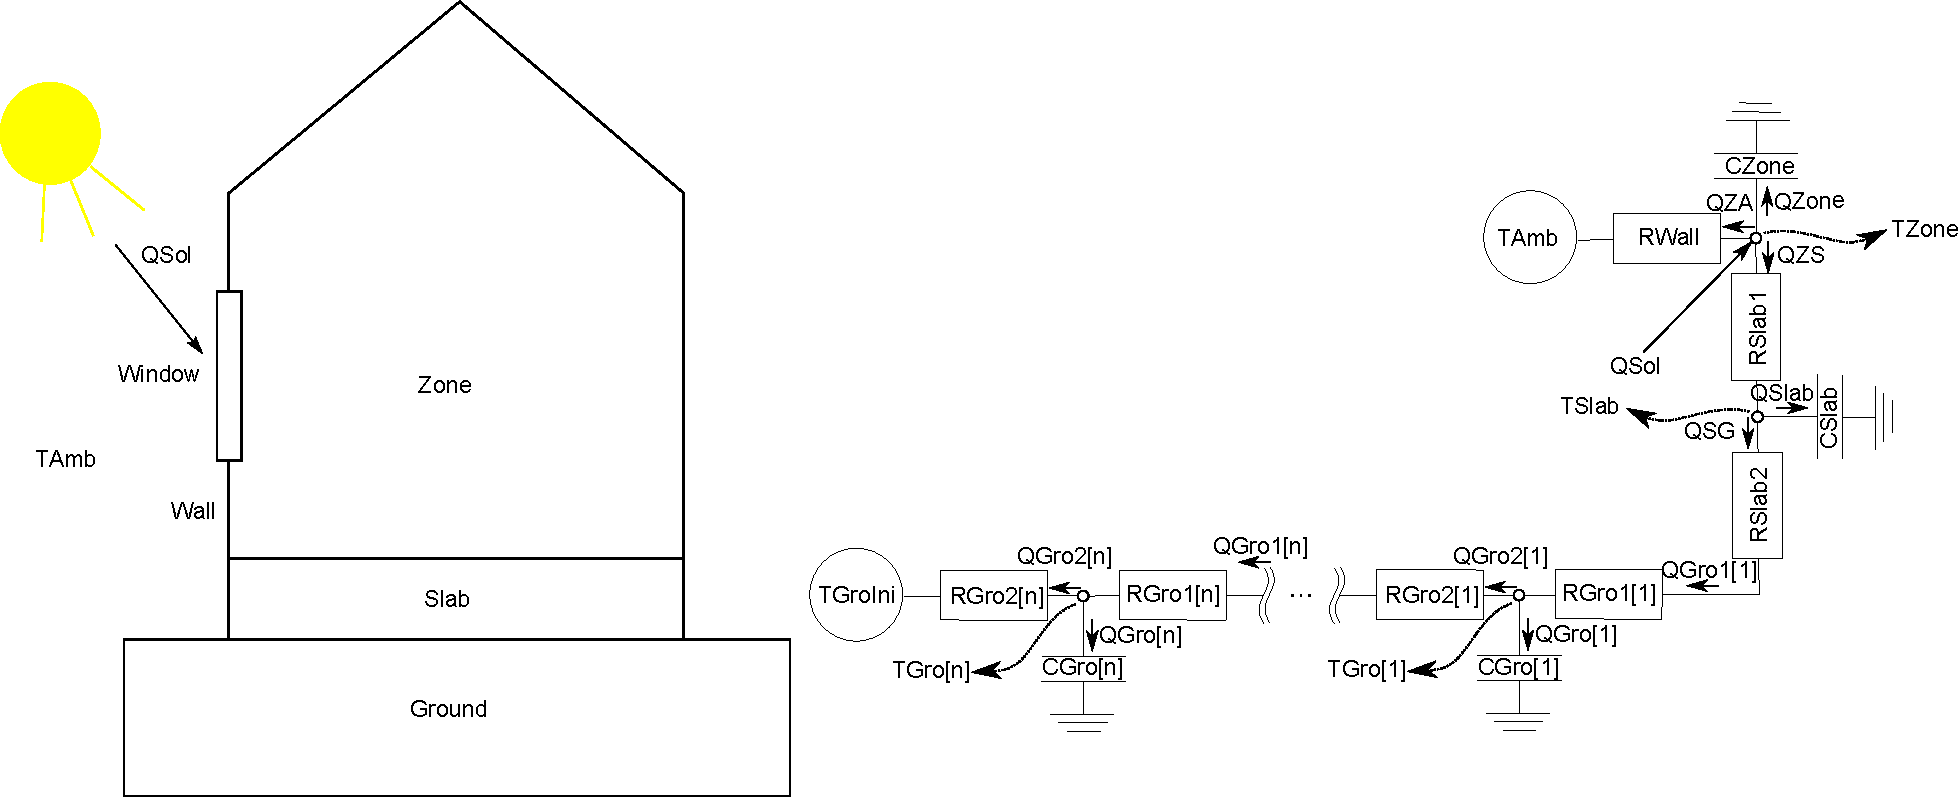
\includegraphics[width=1 \textwidth]{images/RCModelHouse.pdf}
	\caption{ Building model.}
	\label{fig:bui}
\end{figure}

\begin{table}[hbtp] 
\begin{tabular}{cccccc}
\hline 
  & RWall & RSlab1 & RSlab2 & RGro1[i] & RGro2[i] \\  
Thermal resistance $[K/W]$ & 0.00806 & 0.016 & 0.016 & 0.033 & 0.033 \\ 
\hline\hline 
  & CZone & CSlab & CGro[i] &   &   \\  
Thermal capacities $[J/K]$ & $2.4096 * 10^8$ & $3.36 * 10^8$ & $2.52*10^8$ &   &   \\ 
\hline\hline
  & TGroIni & TGro[i](start) & TSlab(start) & TZone(start)&  \\  
Temperature $[K]$ &  283.15 & 283.15 & 293.15 & 293.15 & \\ 
\hline 
\end{tabular} 
\caption{ Building parameters.}
\label{tab:par}
\end{table}

%\newpage
\textbf{Thermal resistance}: $T_1 - T_2 = \text{R} \ Q_{1 \rightarrow 2} $ with $R$ the thermal resistance between node 1 and 2 and $Q_{1\rightarrow 2}$ the heat flow, positive defined from 1 to 2.

\textbf{Thermal capacity}: $C \frac{\text{dT}}{dt} = Q$ with $C$ the thermal capacity and $Q$ the heat flow, positive defined flowing to the capacity.

\textbf{Conservation of energy (Kirchhoff)}: $ \sum Q_i = 0$ or the sum of the heat flows through one node is zero.

\subsection*{Questions}

\begin{enumerate}
\item Apply what you have learned during your reading by setting up a model for the building using the above mentioned equations. Approximate the ambient temperature by a sine using following code: $TAmb = 10*\cos(2*3.14*\text{time}*3*10^\wedge(-8)) + 276.15$ and the solar radiation by a trimmed cosine using: $QSol = \text{floor}(cos(2*\text{Modelica.Constants.pi}*\text{time} / 86400) + 1) * 5000 * cos(2*\text{Modelica.Constants.pi*time} / 86400)$. What is the zone temperature after a year under these conditions?
\item (OPTIONAL): Try to obtain the same results using the components of the Modelica library instead of writting the equations yourself. This library is automatically loaded in Dymola and can be found on the left-hand side of the dymola window. For thermal components, look in the Library at Modelica.Thermal.HeatTransfer.Components.   \linebreak[10]
\end{enumerate}

\begin{center}
 \textbf{Good luck!}
\end{center}

\subsection*{Further reading}
\begin{itemize}
	\item \url{http://simulationresearch.lbl.gov/modelica/downloads/workshops/2015-06-22-lbnl/slides/modelica-intro.pdf}
	\item \url{http://book.xogeny.com}
\end{itemize}

\end{document}
